\chapter{Evaluation}\label{chapter:eval}
\section{Setup}
All benchmarks are run on a system with an Intel Xeon E5-2660 with 251GiB of RAM running Ubuntu 23.10 with a 1TB Samsung Evo 970 Plus NVMe SSD; the throughput and bandwidth limits of the SSD are noted in \autoref{tab:evoplus}.

\begin{table}
    \centering
    \begin{tabular} { ||c|c|c|| }
        \cline{1-3}
        Sequential read & \multicolumn{2}{|c||}{3500 MB/s} \\ \cline{1-3}
        Sequential write & \multicolumn{2}{|c||}{3300 MB/s} \\ \cline{1-3}
        \multirow{2}{*}{Queue Depth 1, Thread 1} & Random read & 19000 IOPS \\ \cline{2-3}
                                                    & Random write & 60000 IOPS \\ \cline{1-3}
        \multirow{2}{*}{Queue Depth 32, Thread 4} & Random read & 600K IOPS \\ \cline{2-3}
                                                    & Random write & 550K IOPS \\ \cline{1-3}
    \end{tabular}
    \caption{Samsung Evo 970 Plus performance limits as per the datasheet}
    \label{tab:evoplus}
\end{table}

In the following sections we will compare our driver's performance with the datasheet numbers in \autoref{tab:evoplus}, as well as against other storage engines: \texttt{libaio}, \texttt{io\_uring}, SPDK and the Linux file I/O API \texttt{pread}/\texttt{pwrite} (\texttt{psync}). Each I/O engine is tested by running a read or write workload over 900 seconds, with I/O unit sizes of 4KiB.

The NVMe controller is aware when a device is empty and thus processes read requests without actually performing any read operations. On an empty drive, the reported read performance will be much higher, hence all read tests are done on a full drive, i.e. each logical block address (LBA) has been written to at least once.

For writes, the SSD is cleared beforehand, such that it is in a comparable state for each test. Full NVMe SSDs report worsened write performances, due to mechanisms such as wear-levelling and write amplification, where the NVMe controller performs garbage collection and reorders data internally.

\section{Throughput}
In this section, we will analyse the throughput capabilities of our NVMe driver, and how changing parameters affects the performance.

Observing the trend of the throughput over time in \autoref{fig:vroom-iops-time}, we the write throughput begin at a heightened rate, at around 800 thousand IOPS (KIOPS) and after approx. 40 seconds decreasing to approx. 200 KIOPS. The SSD has a so-called ``TurboWrite'' buffer region of 42GB, allowing for higher write throughputs, so long the buffer is not fully saturated. On the other hand, read throughput stays relatively constant throughout the entire test, at around 440 KIOPS.

\begin{figure}
  \centering
    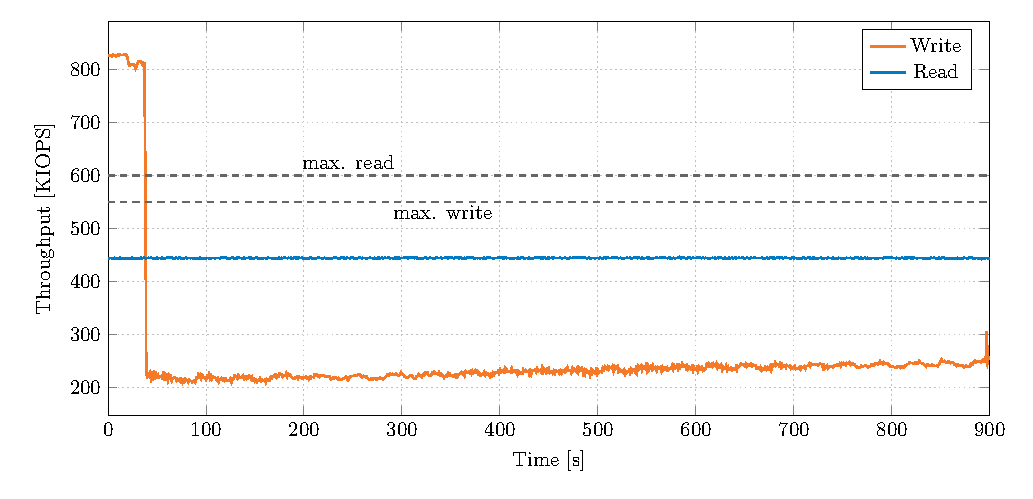
\includegraphics[width=\textwidth]{figures/vroom-iops-time}
    \caption{Throughput over time, QD32T4}
    \label{fig:vroom-iops-time}
\end{figure}

To investigate the effects the number of threads and queue depth (QD) have on throughput, we performed multiple tests with different parameters on the read throughput rather than write to minimize variance.

Observing how the number of threads impact the throughput in \autoref{fig:vroom-iops-thread}, we see the throughput double each time we double the number of threads until 16 threads, afterwards we see gains are smaller. With a queue depth of 32, we see an increase in throughput until 8 threads, after which the throughput plateaus at around 460 KIOPS.

When increasing the queue depth, we notice a similar growth where the IOPS doubles each time the queue depth doubles in size until QD16, however at QD64 the throughput is higher than at 64 threads by approx. 80 KIOPS. Increasing queue depth seems to lead to slightly better performance than increasing the threads when comparing ``queue depths'', i.e. QD32T4 ($\approx$ QD32 $\cdot$ 4) has a lower throughput than QD128T1.

\begin{figure}
  \centering
  \subcaptionbox {Queue depth 1} {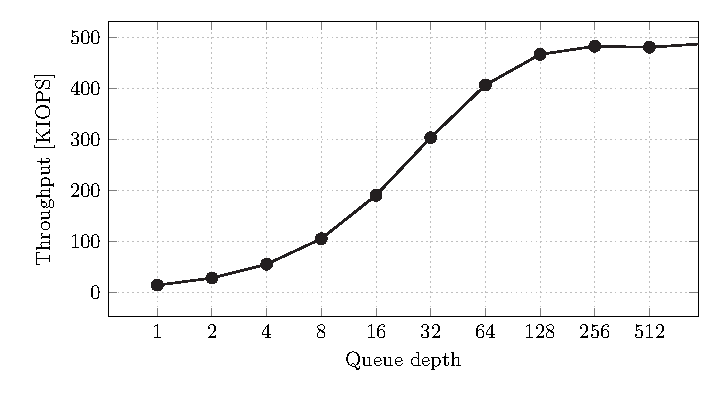
\includegraphics[width=0.48\textwidth]{figures/vroom-iops-qd} \label{fig:vroom-iops-thread-qd1}}
  \subcaptionbox {Queue depth 32} {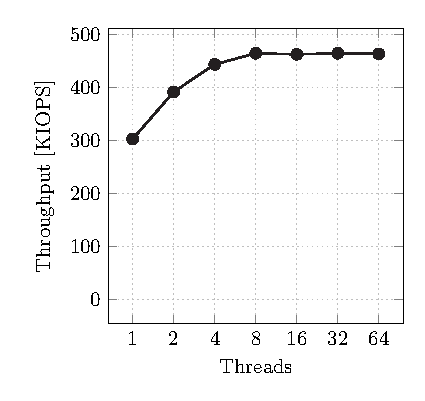
\includegraphics[width=0.48\textwidth]{figures/vroom-iops-thread-qd32} \label{fig:vroom-iops-thread-qd32}}
  \caption{Threads vs. IOPS}
  \label{fig:vroom-iops-thread}
\end{figure}

\begin{figure}
  \centering
  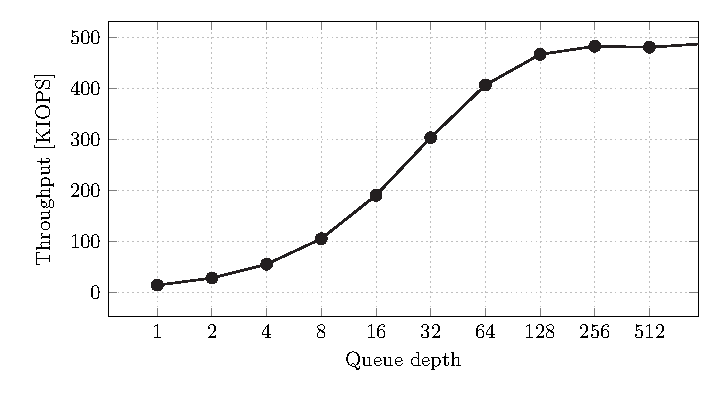
\includegraphics[width=0.48\textwidth]{figures/vroom-iops-qd}
  \caption{Queue depth vs. IOPS}
  \label{fig:vroom-iops-qd}
\end{figure}

% \section{Latency}

\section{Comparison with other I/O engines}
\texttt{libaio}, \texttt{io\_uring} and \texttt{psync}, and in some cases SPDK are tested using \texttt{fio}\footnote{\url{https://github.com/axboe/fio}} with the configuration in \autoref{lst:fio_conf}. In \autoref{fig:iops-qd1}, \autoref{fig:iops-qd32} we use numbers from SPDK's own \texttt{spdk\_perf\_tool} tool, as their \texttt{fio} plugin introduces some overhead; for \autoref{fig:ccdf}, \autoref{fig:lat-qd1} we use log files \texttt{fio} creates.

We use the \texttt{fio} configuration in \autoref{lst:fio_conf}. The same parameters were used when testing with \texttt{spdk\_perf\_tool}.

\begin{lstlisting}[float, label=lst:fio_conf, caption=\texttt{fio} configuration]
  [global]
  io_engine={spdk,io_uring,libaio,psync}
  rw={randread,randwrite,read,write}
  blocksize=4k
  direct=1
  norandommap=1
  runtime=900

  numjobs={1,4}
  queue_depth={1,32}
  group_reporting=1
\end{lstlisting}

\subsection{Queue depth 1}
Here we test the single-threaded read and write performances when using a queue depth of 1, i.e. synchronous read and writes.

\begin{figure}
  \centering
    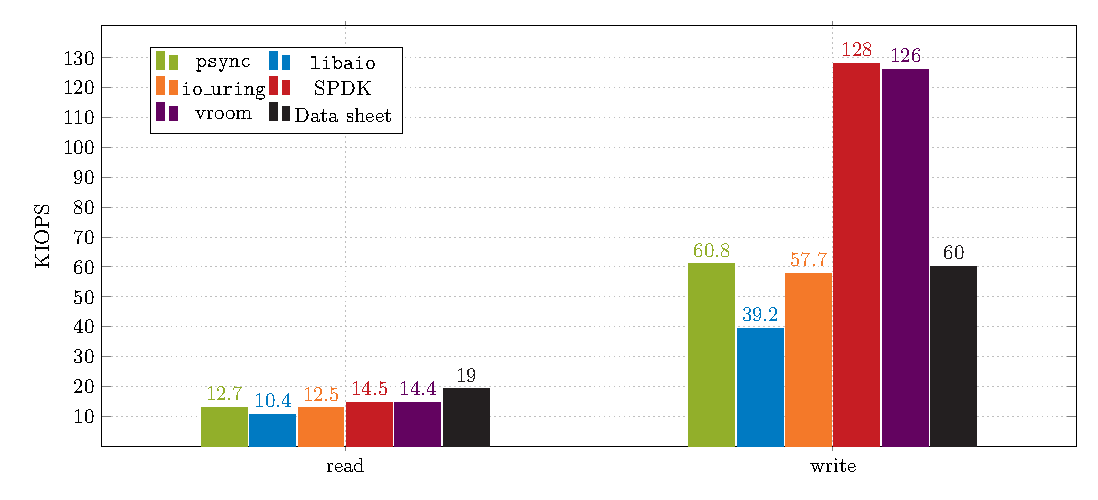
\includegraphics[width=\textwidth]{figures/iops-qd1-ybar}
    \caption{QD1 Throughput}
    \label{fig:iops-qd1}
\end{figure}

Looking at read throughput in \autoref{fig:iops-qd1}, none of the I/O engines come within 20\% of the maximum achievable IOPS of the SSD, performing between 10 and 15 KIOPS. In terms of write performance, we see \texttt{psync} and \texttt{io\_uring} right around 60 KIOPS, while \texttt{libaio} performing considerably below the limit of the SSD. Both SPDK and vroom achieve IOPS numbers doubling the limit stated by Samsung, at 128 KIOPS and 126 KIOPS, respectively.
As Samsung has not specify the test parameters and environment used, it is likely they did not perform these read tests on a fully utilized drive and write test on an empty one. This means they would likely expect higher IOPS than what we observe, as the NVMe controller would not actually access the unwritten areas, increasing the overall IOPS number. While for writes the NVMe controller performs garbage collection when overwriting non-empty areas, introducing some overhead, and thus overall less IOPS.

Comparing I/O engines against one another, we would expect the user space drivers to achieve higher throughput numbers than the rest, which is exactly the result we observe. SPDK and our driver achieve IOPS numbers within 1\% of another, while being noticeably more performant than the Linux I/O APIs, especially when writing. This difference is caused by system calls and the consequent context switches. This is especially visible in \autoref{fig:ccdf}, where the tail distribution of the I/O latencies is plotted; here all I/O engines share a similar distribution, however offset by a certain amount. The system call overhead from \texttt{psync} and \texttt{io\_uring} introduces around 10$\mu$s over SPDK and vroom, while \texttt{libaio} seemingly has some extra internal overhead adding an additional 10$\mu$s to the latencies.

\begin{figure}
  \centering
  \subcaptionbox {Random read} {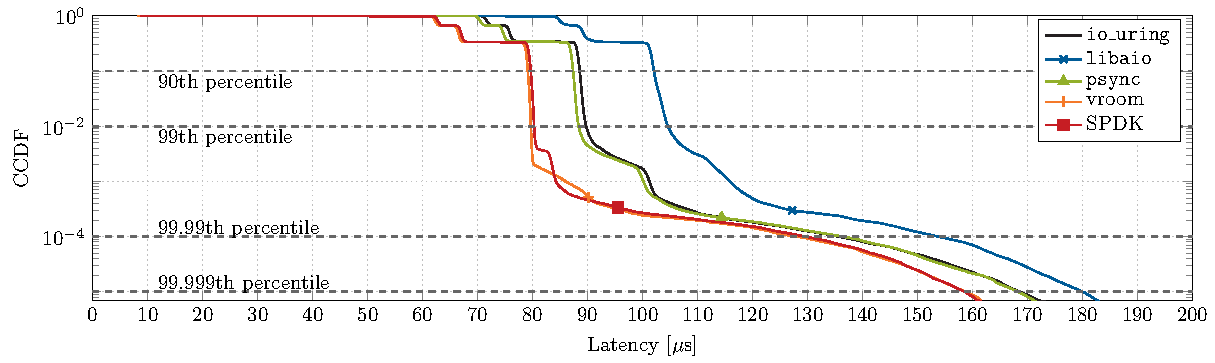
\includegraphics[width=\textwidth]{figures/latency-ccdf-read} \label{fig:ccdf-read}}
  \subcaptionbox {Random write} {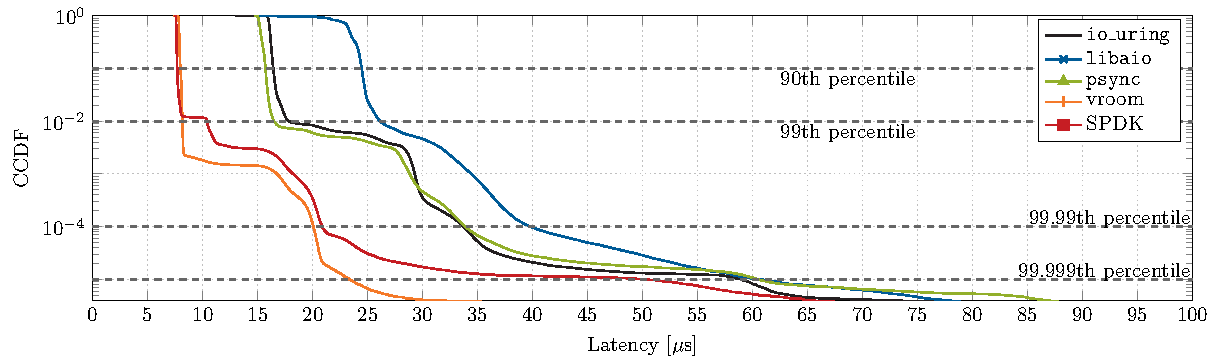
\includegraphics[width=\textwidth]{figures/latency-ccdf-write} \label{fig:ccdf-write}}
  \caption{QD1 latency tail distributions}
  \label{fig:ccdf}
\end{figure}

\begin{figure}
  \centering
  \subcaptionbox {Random read} {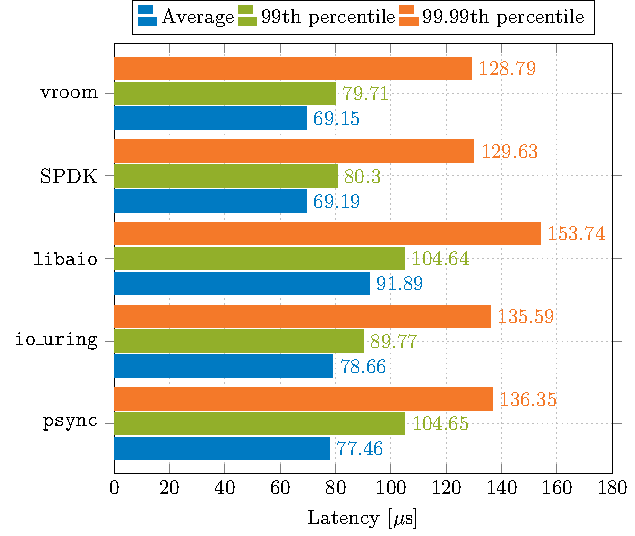
\includegraphics[width=0.48\textwidth]{figures/latency-read-xbar} \label{fig:lat-read}}
  \subcaptionbox {Random write} {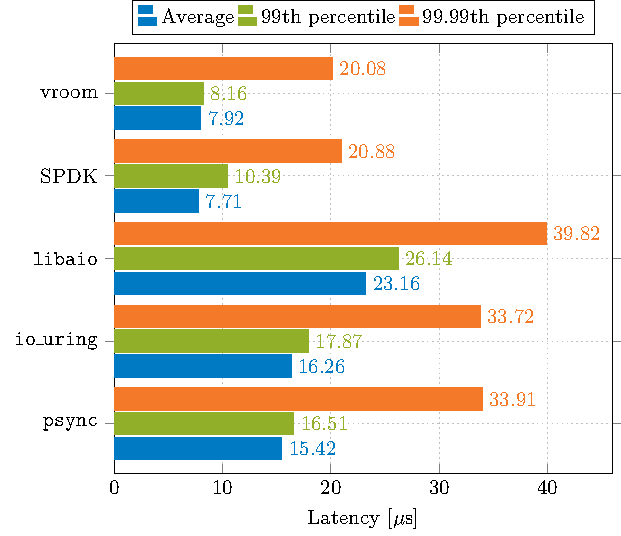
\includegraphics[width=0.48\textwidth]{figures/latency-write-xbar} \label{fig:lat-write}}
  \caption{QD1 latency comparison}
  \label{fig:lat-qd1}
\end{figure}

\subsection{Queue depth 32, Multi-threaded}
Here we tested multi-threaded read and write performances when using a queue depth of 32, without explicitly batching requests; more specifically we used 4 threads, each with a queue depth of 32. \texttt{psync}, as it only allows synchronous I/O, cannot be tested with these parameters.

\begin{figure}
  \centering
    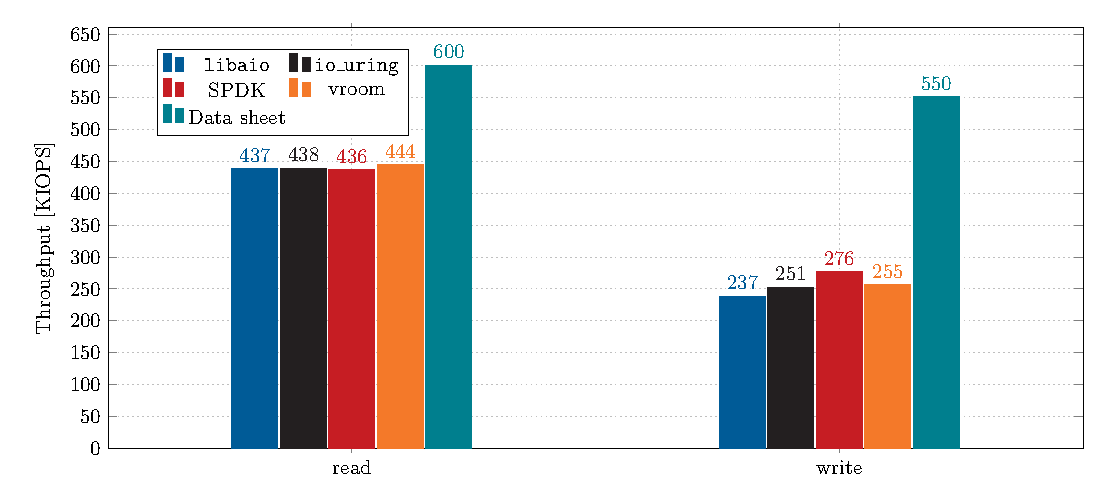
\includegraphics[width=\textwidth]{figures/iops-qd32-ybar}
    \caption{QD32T4 Throughput}
    \label{fig:iops-qd32}
\end{figure}

Like in the previous test, all storage engines perform quite closely in terms of read, here all within 1\% of one another, with vroom being the most performant at 444 KIOPS; however none coming close to the QD32T4 600 KIOPS limit in the datasheet. Interestingly, once we introduce deeper queues and multithreading, the system call overhead does not affect \texttt{libaio} and \texttt{io\_uring} to the same degree as for synchronous I/O when reading.

For random writes, we see \texttt{libaio} yet again falling behind the other I/O engines, but all achieve similar throughputs over the 900 seconds. As we have already observed in \autoref{fig:vroom-iops-time}, the overall write throughput decrease immensely once the SSD's write buffer is saturated, so when we look how the throughput changes over time in \autoref{fig:iops-time-all}, we see SPDK and vroom both clearly ahead in terms of peak throughput, achieving around 800 KIOPS, while \texttt{io\_uring} and \texttt{libaio} have a throughput of approx. 570 KIOPS and 500 KIOPS, respectively. Once the ``TurboWrite'' buffer is fully saturated, the SSD becomes the bottleneck, where each I/O engine perform nearly identically with a throughput of around 220 KIOPS. It is noteworthy that the throughput has a slow increase between the point the SSD is the bottleneck and the end, starting at approx. 200 and ending at 240 KIOPS. Also note that \autoref{fig:iops-time-all} uses IOPS logs from \texttt{fio}, so realistically the throughput of SPDK would likely be higher than vroom initially.

\begin{figure}
  \centering
    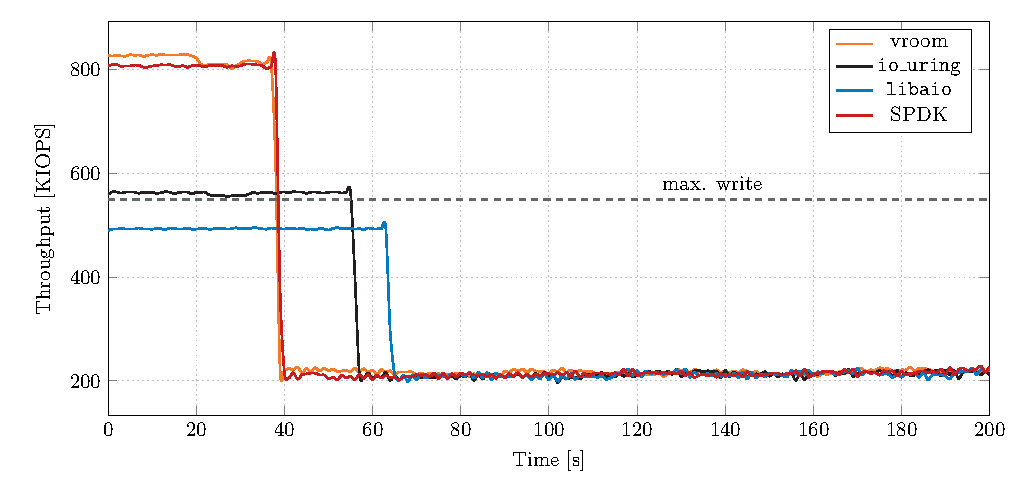
\includegraphics[width=\textwidth]{figures/iops-time-tmp}
    \caption{QD32T4 write throughput development over time of each storage engine}
    \label{fig:iops-time-all}
\end{figure}


\subsection{Summary}
In summary, in these benchmarks we observe that our driver is able to achieve very similar performance and in some cases even better performance than SPDK, while outperforming the kernel based I/O APIs across the board. Overall the poll-based, user space NVMe drivers can reach much higher maximum throughput, while minimising overall I/O latencies by avoiding the kernel altogether.
